\section{Experiments}
\label{sec:experiments}

\paragraph{Data and protocol.} We use RFCx rainforest soundscapes
\citep{rfcx_frugalai} with chainsaw and background labels from four sites carrying enough of both for a per-site
estimate: warsi ($412$ chainsaw / $198$ background test clips), tambopata
($41/72$), romania ($30/15$), pooks ($10/12$). Every experiment is
\emph{leave-one-site-out}: all clips from the target site are reserved for test,
everything is fit on the remaining sites, and the decision threshold is
calibrated on a training-site background validation split at a background
false-positive budget of $0.10$. A recording-level audit confirms zero clips from
the held-out site in train or validation and zero shared source recordings across
splits, so no result below is contaminated by clip-window leakage.

\paragraph{Metrics.} \emph{Flagged recall} (positives scoring above threshold),
\emph{attributed recall} (flagged \emph{and} the predicted kind is correct),
\emph{background FP}, and threshold-free AUC of the score separating chainsaw
from background. For the supervised probe we additionally report
\emph{event-level recall}: clips are grouped back into source recordings and an
event counts as detected if any of its clips fires, since a chainsaw runs
continuously and the operational unit is the event, not the $3$-second clip.

\paragraph{Implementation and reproducibility.} The detector and evaluation math
are NumPy and unit-tested ($123$ tests); audio inference uses PyTorch~2.7 with
\texttt{panns\_inference} (AudioSet CNN14, $2048$-d) and \texttt{birdnetlib}
(BirdNET V2.4, $1024$-d) on CPU/Apple-Silicon under macOS. Randomized results fix
seeds and every interval is a $1000\times$ bootstrap. All numbers below were
regenerated from scratch for this submission; code, fitted artifacts, manifests,
and the exact commands are released. The evaluation audio is public and released
under CC BY-NC 4.0; the closed-set lineage additionally trains on public forest
and urban corpora \citep{bandara2023fsc22,gemmeke2017audioset}.

\subsection{From diagnosis to a deployable operating point}

Section~\ref{sec:diagnosis} established that closed-set classifiers fail across
sites through operating-point transfer and site encoding. Table~\ref{tab:headline}
compares, on the primary held-out site, the strongest closed-set baseline against
the open-set detector under two embeddings. The closed-set model is a CNN trained
on rainforest audio \emph{with tambopata held out}, the most favorable closed-set
setting: $0.976$ chainsaw recall at raw argmax, but with half of all background
flagged as a threat; calibrated to a deployable false-positive rate, recall
collapses to $0.195$. Re-using that same CNN as the open-set \emph{embedding}
inherits the site bias, giving an anomaly-score AUC of $0.319$, below chance, and
consistent with the representation analysis in Section~\ref{sec:diagnosis}.
Swapping in a frozen AudioSet encoder is what recovers a usable operating point.

\begin{table}[t]
\centering
\caption{Held-out-site (tambopata) chainsaw detection, threshold calibrated to
background FP $\le 0.10$ on training-site validation. All rows are our own
re-run under one protocol. ``Score AUC'' is threshold-free separability
\emph{before} any labels are used.}
\label{tab:headline}
\small
\begin{tabular}{lrrr}
\toprule
Method & Recall & Bg FP & Score AUC \\
\midrule
Closed-set CNN (raw argmax)       & 0.976 & 0.500 & --- \\
Closed-set CNN (calibrated)       & 0.195 & 0.000 & --- \\
Open-set, site-trained CNN        & 0.049 & 0.028 & 0.319 \\
Open-set, AudioSet CNN14          & \textbf{0.317} & 0.056 & \textbf{0.713} \\
\bottomrule
\end{tabular}
\end{table}

\begin{table}[t]
\centering
\caption{Leave-one-site-out folds, open-set (background-only) detector.
The AudioSet embedding lifts separability above chance at every site where the
site-trained CNN is at or below it, but the validation-calibrated threshold does
not always hold the FP budget on an unseen site. pooks has only $10$ held-out
chainsaw clips and should be read as indicative.}
\label{tab:folds}
\small\setlength{\tabcolsep}{4pt}
\begin{tabular}{lrrrrr}
\toprule
& & \multicolumn{2}{c}{site-trained CNN} & \multicolumn{2}{c}{AudioSet CNN14} \\
\cmidrule(lr){3-4}\cmidrule(lr){5-6}
Site & $n_{\text{ch}}$ & Recall & AUC & Recall & AUC \\
\midrule
tambopata & 41  & 0.049 & 0.319 & 0.317 & \textbf{0.713} \\
warsi     & 412 & 0.250 & 0.481 & 0.367 & 0.619 \\
romania   & 30  & 0.167 & 0.564 & 0.267 & 0.559 \\
pooks     & 10  & 0.000 & 0.146 & 0.000 & 0.546 \\
\bottomrule
\end{tabular}
\end{table}

\subsection{The representation, not the head, governs transfer}

Because the open-set machinery is identical across embeddings, the comparison
isolates the effect of the frozen encoder $\phi$. The site-trained CNN inherits
the domain bias that sinks the closed-set model (AUC $0.15$--$0.56$, at or below
chance), whereas the frozen AudioSet encoder is above chance at every held-out
site ($0.55$--$0.71$; Table~\ref{tab:folds}). On the primary site it reaches
$0.317$ flagged recall at $0.056$ background FP, exceeding the closed-set
calibrated recall of $0.195$ while using \emph{zero} labeled positives to decide
what is anomalous.

Two caveats temper this. Absolute recall is modest ($0.27$--$0.37$ where the FP
budget is met): faint, distant chainsaws under an unseen chorus remain hard.
And the threshold calibrated on training-site background does not always hold the
budget on an unseen site (warsi $0.20$, romania $0.13$), a cross-site
\emph{calibration} gap distinct from the separability the embedding provides.

\subsection{What label-free operation costs}
\label{sec:cost}

To separate what is lost by using no labels from what is lost to site shift, we
fit a supervised probe (logistic regression) on the \emph{same} frozen embeddings
using the training-site chainsaw labels a real deployment eventually accumulates,
under the identical leave-one-site-out protocol and FP budget
(Table~\ref{tab:probe}, Figure~\ref{fig:transfer}). This is the label-rich upper
bound for a given representation.

\begin{table}[t]
\centering
\caption{Supervised leave-one-site-out probe over frozen embeddings, at the same
$0.10$ background-FP budget. AUROC is threshold-free, event recall groups clips
into source recordings. Rows are $n$-weighted means over the four folds; per-site
AUROC $95\%$ CIs are bootstrap. The choice of representation moves transfer far
more than the choice of head.}
\label{tab:probe}
\small
\begin{tabular}{lrrr}
\toprule
Frozen embedding & AUROC & Clip recall & Event recall \\
\midrule
site-trained CNN & 0.648 & 0.369 & 0.370 \\
AudioSet CNN14   & 0.783 & \textbf{0.594} & \textbf{0.595} \\
BirdNET V2.4     & \textbf{0.786} & 0.527 & 0.531 \\
\bottomrule
\end{tabular}
\end{table}

\begin{figure*}[t]
\centering
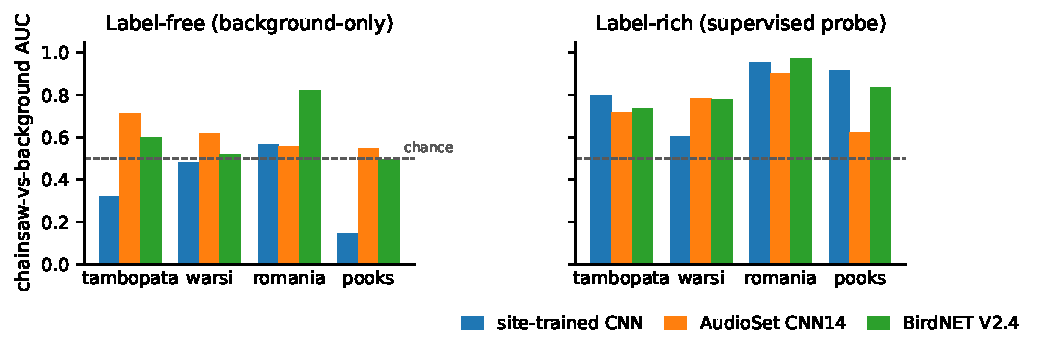
\includegraphics[width=\textwidth]{figures/transfer.pdf}
\caption{Per-site chainsaw-vs-background AUC, label-free (left) and label-rich
(right), for the three frozen embeddings. Dashed line is chance. General-purpose
audio representations transfer; the site-trained one does not.}
\label{fig:transfer}
\end{figure*}

Three findings follow. First, the general-purpose encoders are far better
substrates than the site-trained CNN: weighted AUROC $0.783$ (AudioSet) and
$0.786$ (BirdNET) against $0.648$, and on romania BirdNET reaches AUROC $0.973$
with $0.966$ event recall at $0.067$ FP, an operationally useful detector.
Second, the two general encoders are near-tied on AUROC despite very different
pretraining (AudioSet tagging versus bird vocalization), which points to generic
acoustic generality rather than any threat-specific prior as the active
ingredient. Third, comparing Table~\ref{tab:probe} with Table~\ref{tab:folds}
prices label-free operation: with labels, the AudioSet representation supports
$0.594$ event recall; without them, background-only flagging on the same
representation delivers $0.317$ on the primary site. Labels roughly double
recall, but the label-free detector is the one that can run on day one.

\subsection{Ranking can be strong while calibration fails}

BirdNET makes the paper's central distinction unusually sharp. As a supervised
probe it is the best embedding we tested (weighted AUROC $0.786$). Yet under
the label-free detector it flags \emph{nothing} at every site (recall $0.000$),
despite threshold-free AUC up to $0.821$ on romania. The score ranks chainsaws
above background; the background-density threshold calibrated on training sites
simply lands in the wrong place on an unseen one. This is the same
operating-point failure we diagnosed in the closed-set classifier
(Section~\ref{sec:diagnosis}), reappearing in a fully unsupervised detector, and
it is why we report recall at a fixed FP budget rather than AUC alone: an
embedding can be excellent and still be undeployable if its operating point does
not transfer.

\subsection{Attribution lights up with a handful of labels}

Figure~\ref{fig:kcurve} plots attributed recall against the number of verified
positives per class $k \in \{0,1,5,10,25\}$, with flagging held fixed. At $k=0$
every anomaly is honestly unknown by construction ($0.000$ attributed recall); on
tambopata attribution rises to $0.112$ at $k=5$ and $0.180$ at $k=25$. Flagging
is identical across all $k$ by construction, so ranger confirmations only move
mass from \emph{unknown} onto the named class, which is the day-one-useful,
self-improving behavior a human-in-the-loop deployment needs.

\begin{figure}[t]
\centering
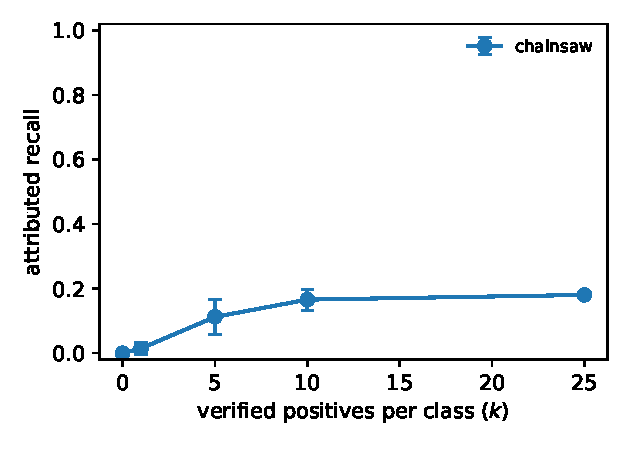
\includegraphics[width=0.85\columnwidth]{figures/kcurve.pdf}
\caption{Attributed recall vs.\ verified positives per class (tambopata
held-out, AudioSet embedding; mean $\pm$ std over seeds). Flagging is independent
of $k$; only attribution depends on it.}
\label{fig:kcurve}
\end{figure}

\subsection{Honest unknowns}

To test abstention we remove chainsaw's prototype entirely and re-score the
held-out site's chainsaw clips. A well-behaved open-set detector should still
\emph{flag} them, since they remain acoustically unusual, while assigning their
likelihood mass to \emph{unknown} rather than misattributing it to a remaining
class. This is what we observe: flagging is unchanged and $100\%$ of flagged
clips are predicted \emph{unknown} with mean unknown mass $1.0$. The detector
never invents a label for a class it was never shown.

\subsection{Limitations}

Our evidence is one threat class (chainsaw) across four rainforest sites, and two
folds are small ($n=30$ and $n=10$), so per-site numbers carry wide intervals and
we weight by $n$ when aggregating. Absolute label-free recall remains modest, and
the calibration gap means an operator should expect to spend a small amount of
destination-site background to place the threshold. We evaluate on recorded
clips, not a live deployment; a field study with in-situ positives is the
necessary next step and is underway.
